\documentclass[14pt]{extarticle}

\usepackage{fontspec}
\setmainfont{Times New Roman}

% размер полей
\usepackage{geometry}
\geometry{a4paper, top=2cm, bottom=2cm, right=1.5cm, left=3cm}

 %debugging
%\usepackage{showframe}

% полуторный интервал
\usepackage{setspace}
\onehalfspacing

% абзацный отступ
\setlength{\parindent}{1.25cm}

% выравнивание текста по ширине
\sloppy

% списки
\usepackage{calc} % арифметические операции с величинами
\usepackage{enumitem}
\setlist{
    nosep,
    leftmargin=0pt,
    itemindent=\parindent + \labelwidth - \labelsep,
}

% подписи к рисункам и таблицам
\usepackage{caption}
\renewcommand{\figurename}{Рисунок}
\renewcommand{\tablename}{Таблица}
\DeclareCaptionFormat{custom}
{
    \textit{#1#2#3}
}
\DeclareCaptionLabelSeparator{custom}{. }
\captionsetup{
    % хз какой это размер - 12 или нет, но выглядит меньше 14
    font=small,
    format=custom,
    labelsep=custom,
}

% картинки
\usepackage{graphicx}

% колонтитулы
\usepackage{fancyhdr}

% картинки и таблицы находятся именно в том месте текста где помещены (атрибут H)
\usepackage{float}

% таблицы
\usepackage{tabularray}

\graphicspath{ {8.2.2/models/} }
\usepackage{hyperref}
\begin{document}
\pagestyle{fancy}
\fancyhead{}
% disable header
\renewcommand{\headrulewidth}{0pt}
\fancyfoot[L]{Дубровских гр 221-361}
\fancyfoot[C]{ЛР 8.2.2}
\fancyfoot[R]{Продажа автотранспорта}
\singlespacing

\newpage
\begin{center}
    Министерство науки и высшего образования Российской Федерации
    Федеральное государственное автономное образовательное учреждение

    высшего образования

    \guillemotleft МОСКОВСКИЙ ПОЛИТЕХНИЧЕСКИЙ УНИВЕРСИТЕТ\guillemotright

    (МОСКОВСКИЙ ПОЛИТЕХ)
\end{center}
\noindent
\bigbreak
\bigbreak
\bigbreak
\bigbreak
\begin{center}
    ЛАБОРАТОРНАЯ РАБОТА 8.2.2

    По курсу Проектирования пользовательских интерфейсов в веб

    \textbf{Прототипирование интерфейса в Figma}
    \bigbreak
    \bigbreak
    \bigbreak
    \bigbreak
    ТЕМА

    \guillemotleft\textbf{САЙТ ДЛЯ ПРОДАЖИ И ПОИСКА АВТОМОБИЛЕЙ}\guillemotright
\end{center}
\noindent
\bigbreak
\bigbreak
\bigbreak
\bigbreak
\bigbreak
\bigbreak
\bigbreak
\bigbreak
\bigbreak
\bigbreak
\hfill Выполнил

\hfill Дубровских Никита Евгеньевич

\hfill Группа 221-361
\bigbreak
\bigbreak
\bigbreak
\hfill Проверил

\hfill Натур ВВ
\vfill
\begin{center}
    Москва, 2024
\end{center}
\newpage
\onehalfspacing


\begin{center}
    \textbf{Лабораторная работа 8.2.2}

    \textbf{Прототипирование интерфейса в Figma}
\end{center}

\textbf{Цель работы:} создать динамический (кликабельный) прототип интерфейса.
\bigskip

\textbf{Задачи:}

\begin{enumerate}
    \item Настроить взаимодействие между экранами и элементами интерфейса в соответствии со сценариями логического взаимодействия.Переходы подключаются в соответствии логическим схемам, Карте сайта и сценариям (блок-схема)
    \item Скачать готовый Wireframe Kit и доработать под свои цели и задачи
    \item Установить анимацию переходов.
    \item Протестировать динамический прототип интерфейса.
\end{enumerate}
\bigskip

\textbf{Основные термины}

\begin{itemize}
    \item Прототип — модель будущего интерфейса сайта или приложения, позволяющая визуализировать структуру и функциональность проекта на начальных этапах разработки. Прототип может быть статичным (LoFi, HiFi) или интерактивным.
    \item Динамический прототип — кликабельный прототип, в котором настроены взаимодействия и переходы между экранами, включая анимации, что позволяет моделировать пользовательский опыт.
    \item Wireframe Kit — набор упрощенных графических элементов для прототипирования интерфейсов, включающий базовые блоки и компоненты для быстрого создания наброска структуры сайта.
    \item Анимация — элемент дизайна, используемый для повышения интерактивности прототипа. Включает три вида: Navigate (переход на новый экран), Swap (замена одного элемента другим), Overlay (наложение всплывающих элементов).
    \item LoFi Wireframe (низкая детализация) — начальный набросок интерфейса, использующий простую разметку блоков, что помогает определить общую структуру без детальных элементов.
    \item HiFi Wireframe (высокая детализация) — статичный прототип с подробной разметкой и наполнением, включая тексты, изображения и графику, создающий представление о визуальном стиле интерфейса.
    \item Интерактивный прототип с высокой детализацией — модель, включающая анимации и поведенческие элементы интерфейса, позволяющая протестировать пользовательские сценарии на разных устройствах.
    \item UI-кит — коллекция стандартных элементов интерфейса (кнопки, поля ввода, иконки и пр.), часто используемых в прототипировании для поддержания единого стиля и ускорения разработки.
\end{itemize}
\bigskip

\textbf{Кликабельный прототип}
\bigskip

\noindent
\begin{minipage}{\linewidth}
    \fbox{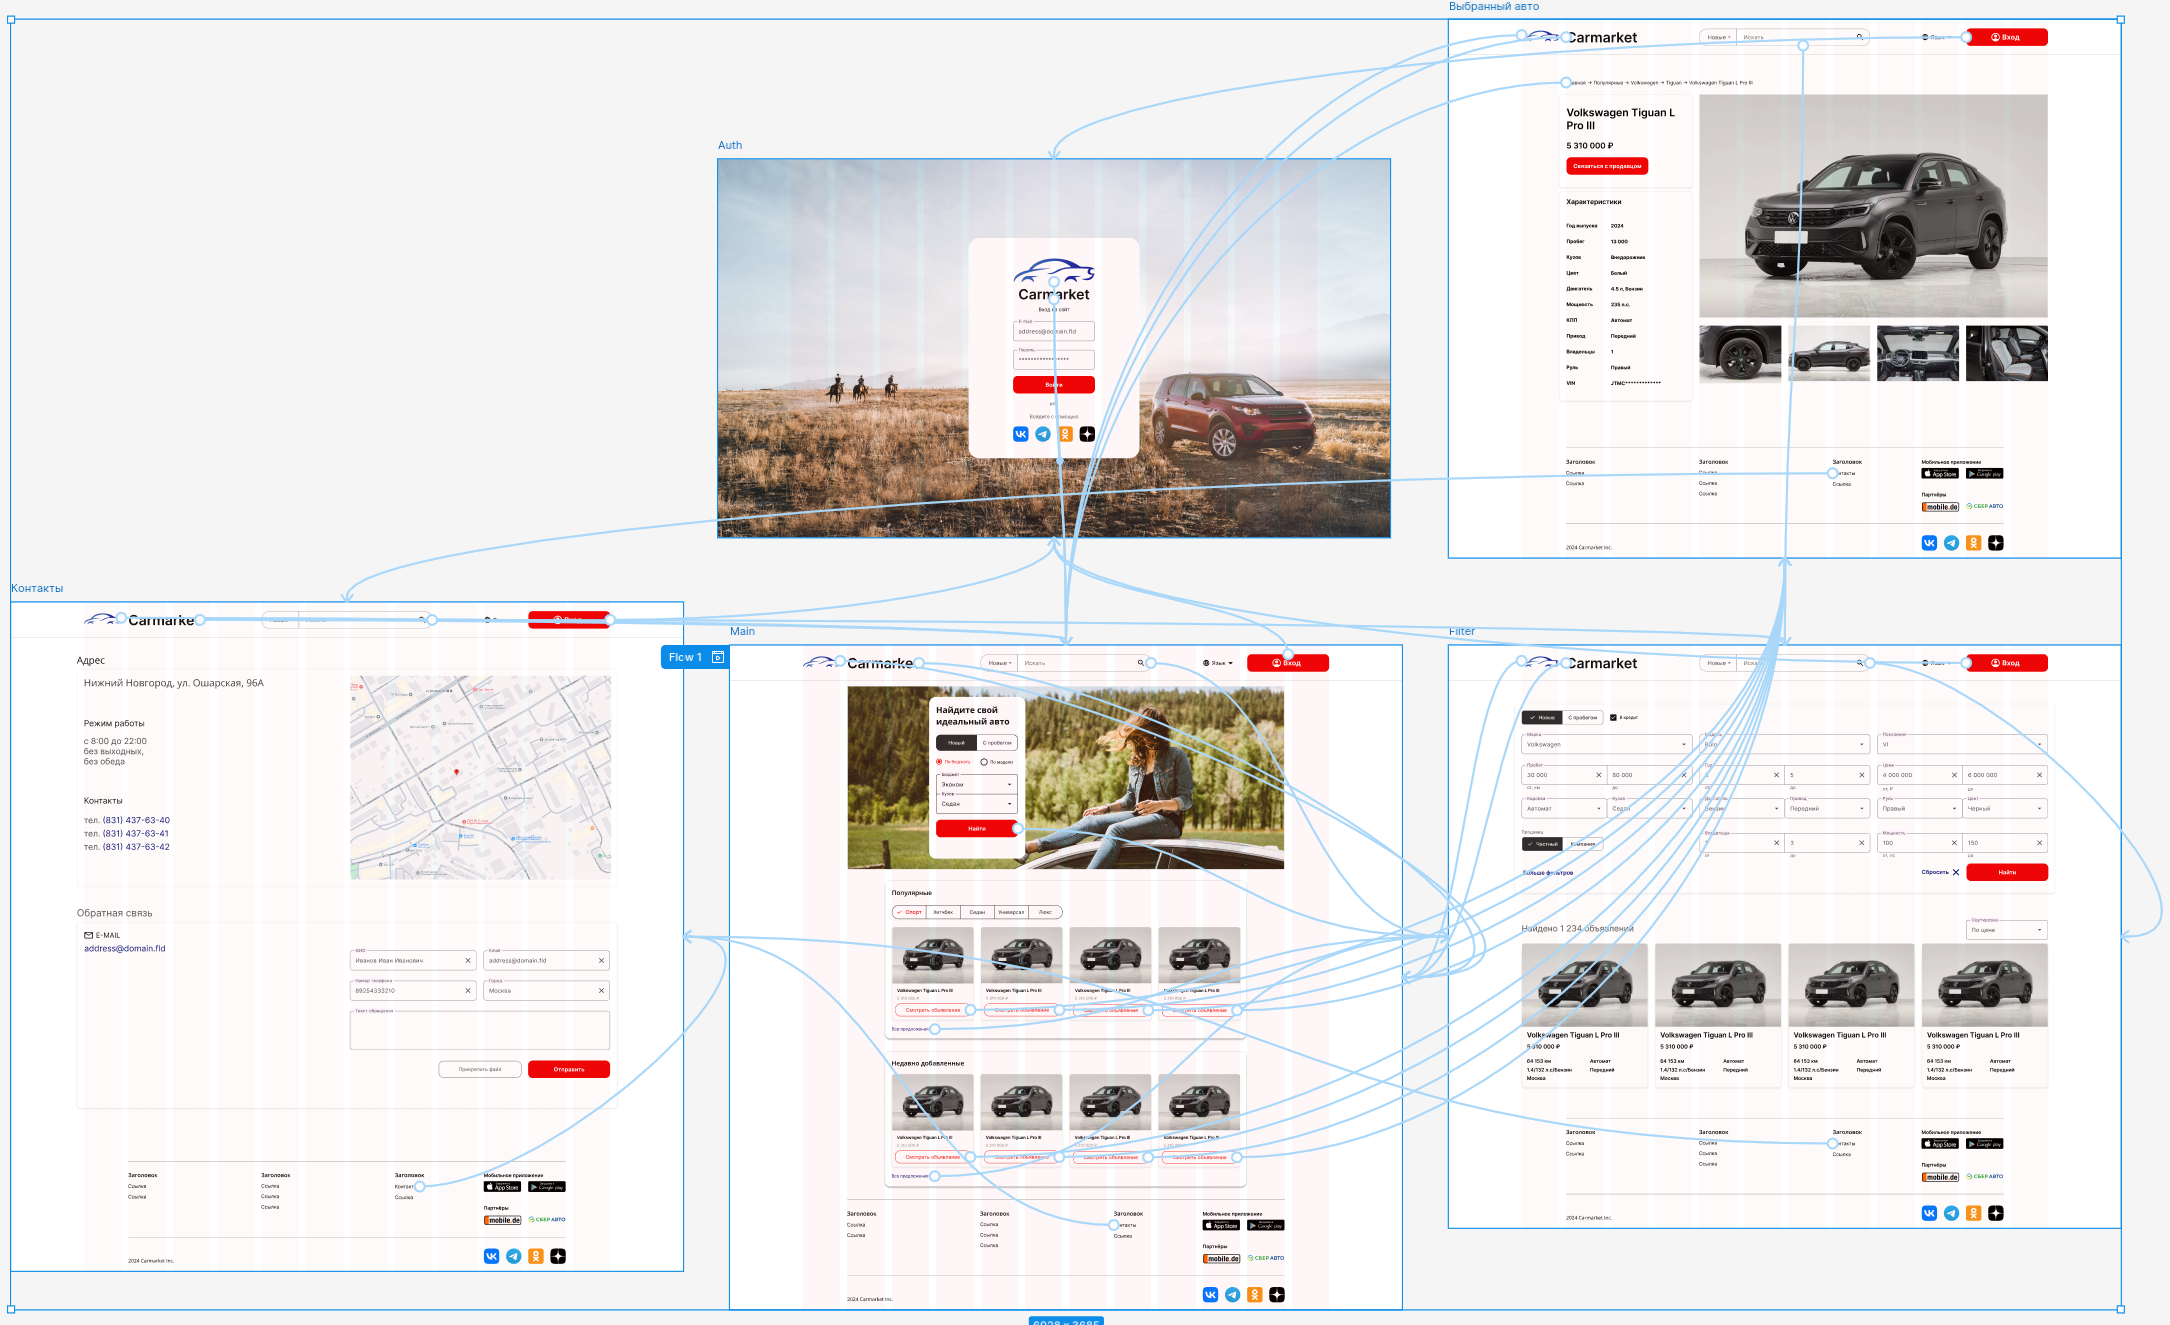
\includegraphics[width=\linewidth]{p}}
\end{minipage}
\bigskip

Ссылка:

\url{https://www.figma.com/design/25STw8qqDFUKFnCIDQb1ri/PPI?node-id=0-1&t=GBgUWcyWpiIqqghb-1}
\bigskip

\textbf{Контрольные вопросы и ответы}

\begin{enumerate}
    \item Что такое прототип сайта?

        Прототип сайта — это предварительная модель веб-ресурса, которая демонстрирует структуру, функциональность и взаимодействие элементов интерфейса. Он помогает визуализировать идею сайта до его разработки, позволяя заказчику и команде разработчиков понять, как будет выглядеть и работать конечный продукт.

    \item Для чего нужен прототип сайта заказчику?

        Прототип сайта необходим заказчику для уточнения требований к проекту, обсуждения и согласования дизайна, а также для более наглядного представления функциональности сайта. Это позволяет избежать недоразумений и недовольства по завершении разработки, так как заказчик может видеть, как его идеи реализуются.

    \item Какие задачи решает прототип сайта для команды разработчиков?

        Прототип помогает команде разработчиков определить структуру и логику взаимодействия элементов интерфейса,
    выявить и устранить недочеты на ранних этапах разработки,
    упростить коммуникацию между участниками проекта, предоставляя наглядный документ для обсуждения,
    сформулировать более точные сроки и оценку стоимости разработки на основе визуализированного представления.

    \item Каковы основные шаги создания прототипа в программном ресурсе Figma?

    Определение цели и задач прототипа,
    создание вайрфрейма (каркасного макета) интерфейса,
    настройка взаимодействия между экранами и элементами интерфейса,
    добавление анимации переходов для улучшения восприятия,
    тестирование прототипа и внесение коррективов.

\item Что такое UI-кит и когда используется?

    UI-кит (User Interface Kit) — это набор готовых элементов интерфейса (кнопок, форм, иконок и т. д.), которые используются для ускорения процесса дизайна. Он позволяет дизайнерам не создавать элементы с нуля, а использовать стандартизированные компоненты, что улучшает согласованность и упрощает работу над проектом.
\end{enumerate}

\end{document}
